\documentclass[11pt]{article}

\title{%
  Analiza poveznica \\ 
  \large Središta i autoriteti na webu }
\author{Bruno Fabuli\'{c}, Helena Marciu\v{s}, Dora Parma\v{c}}


\usepackage{amsmath}
\usepackage{amsthm}
\usepackage{amssymb}
\usepackage{esvect}
\usepackage[utf8]{inputenc}
\usepackage{amsfonts}
\usepackage{hyperref}
%\hypersetup{colorlinks=true}
\newcommand\eref[1]{(\ref{#1})}
\usepackage{enumitem}
\usepackage[croatian]{babel}
\usepackage{graphicx}
\graphicspath{ {./images/} }
\hypersetup{
    urlcolor=black
}
\newtheorem{theorem}{Teorem}[section]
\newtheorem{prop}{Propozicija} [section]
\newtheorem{corollary}{Korolar}[theorem]
\usepackage{listings}

\usepackage{biblatex}
\addbibresource{dokumentacija.bib}
\usepackage{csquotes}



\begin{document}
	\maketitle
	\pagenumbering{gobble}
	\newpage
	\hypersetup{linkcolor=black}
	\tableofcontents
	\pagenumbering{roman}
\newpage
\hypersetup{linkcolor=red}
\pagenumbering{arabic}

\section{Uvod}
Budući živimo u svijetu informacija, Internet je dio našeg svakodnevnog žiota, te imamo pristup do više informacija nego što možemo procesuirati. Zbog toga nam je potrebna metoda za filtriranje informacija.
Kao odgovor, javljaju se tehnike za pretraživanje.Njih možemo opisati kao proces koji nam omogućava pretraživanje veće kolekcije dokumenata za specifičnu informaciju koju nazivamo upit (eng. query).

Web je kolekcija dokumenata čije karakteristike ga čine posebno kompleksnim za pretraživanje. Pretraživači su suočeni s problemima kao što je sama veličina Weba, brzina kojom se mijenja i raste, te nedostatkom sustavne organizacije. Procjenjuje se da sadrži preko 45 milijardi stranica što ga čini najvećom kolekcijom dokumenata na svijetu, a to je samo indeksirani dio. Također, dinamičan je (godišnje nastaje milijarde novih dokumenata zbog čega je pretraživačima teško izračunati njihovu relevantnost za postavljeni upit) i nije sustavno organiziran jer svatko može stvoriti stranicu u bilo koju svrhu. Podatci konstantno nastaju i nestaju, a poveznice (eng. link) se stvaraju i pucaju jer odredišta postaju nedostupna.

Kao rješenja danog problema, pojavila se metoda analize poveznica.
Stranice na webu povezane su hipervezama koju se web pretraživačima važan izvor informacija. Korisne su jer označavaju referencu stranice A na stranicu B što samo po sebi nije značajno korisno. No, ako pretpostavimo da autori stranice koriste poveznice za koje misle da će biti korisne čitatelju i ako su to poveznice na kvalitetne stranice koje obogaćuju sadržaj ili podupiru stajališta autora, onda na njih možemo gledati kao preporuku autora stranice A na stranicu B.
Analiza poveznica se uspješno koristi za pronalaženje i indeksiranje novih stranica, rangiranje rezultata pretraživanja, te kategorizaciju web stranica.

\newpage

\section{HITS algoritam}

Jedan od algoritama za rangiranje web stranice ovisno o upitu koje ćemo proučavati je Kleinbergov HITS algoritam. 

Iz grafa poveznica G stvara se manji graf (eng. neighborhood
graph) koji sadržava samo čvorove stranica koje odgovaraju upitu, proširen njihovim 'susjednim' stranicama. Susjedi u ovom slučaju znače set stranica koje poveznicama pokazuju na, ili na njih pokazuju dokumenti iz početnog seta koji odgovara upitu. Takav set stranica može biti jako velik pa se u praksi često ograničava na manji broj prethodnika. Rangiranje se potom vrši prema tom grafu uzimajući u obzir broj linkova vezanih uz čvor svake stranice iz početnog seta. Kao i prije problem je što svaka poveznica vrijedi jednako.
Kod upita, algoritam prvo iterativno računa vrijednost središta (eng. hub score) i vrijednost autoriteta (eng. authority score) za svaki čvor iz grafa susjeda. Dokumenti se onda rangiraju prema obje vrijednosti. 

Za dokumente s visokim autoritetom smatra se da bi trebali imati relevantni sadržaj. Dokumenti središta trebali bi imati poveznice na relevantne dokumente.Ideja je da bi dokumenti koji pokazuju na mnoge druge mogli biti dobra središta, a dokumenti na koje pokazuju mnogi drugi dokumenti dobri autoriteti.

\newpage
\section{WWW kao usmjereni graf}

Svaku kolekciju povezanih web stranica možemo predstaviti usmjerenim grafom $G=(V,E)$. Web stranice predstavljamo vrhovima, tj. $V$ je skup web stranica, a poveznice između stranicama predstavljamo bridovima - za stranice $p_{i}$, $p_{j} \in V$, brid $e_{ij}$ je u $E$ ako postoji poveznica sa stranice $p_{i}$ na stranicu $p_{j}$. Kažemo da je stupanj izlaznosti (out - degree) vrha $p_{i}$ broj vrhova na koje $p_{i}$ pokazuje, a stupanj ulaznosti (in-degree) broj vrhova koji pokazuju na $p_{i}$. \\ 

Kažemo da je vrh i
\begin{itemize}
    \item dobar izvor informacije o lokaciji kvalitetnog sadržaja ili dobro čvorište (hub) ako sadrži  linkove na vrhove koju su dobri autoriteti u smislu sadržavanja kvalitetne informacije
    \item dobar autoritet (sadrže kvalitetnu informaciju o nekoj temi) ako na njega pokazuju dobri hubovi)
\end{itemize}

Dakle, svakom vrhu, odnosno svakoj stranici $p_{i}$ pridružujemo uređen par $(x_{i}, y_{i})$ nenegativnih brojeva kao mjeru za "biti dobar autoritet" i "biti dobar "hub".

\begin{center}
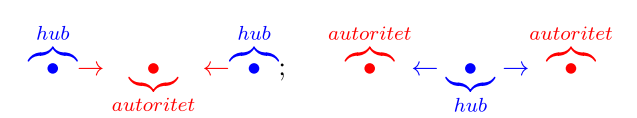
\includegraphics[width= \textwidth]{hubovi.png}    
\end{center}

Težine $x_{i} \geq 0$ i $y_{i} \geq 0$ definirano rekurzivno s:
\begin{equation} \label{eq:1}
x_{i} = \sum_{j: e_{ji}\in E} y_{j} \hspace{1cm}  y_{i} = \sum_{j: e_{ij}\in E} x_{j}
\end{equation}
Odnosno, autoritet-vrijednost web stranice je suma hub-vrijednosti svih stranica koje pokazuju na nju. Hub vrijednost web stranice je suma autoritet-vrijednosti web stranica na koje ona pokazuje.
Intuitivno, smatramo da je web stranica dobar autoritet ako na nju pokazuju dobri hubovi. Analogno, smatramo da je web stranica dobar hub ako pokazuje na dobre autoritete.

\newpage
Kako odrediti $ x_{i}, y_{i} $ ?

Stavimo $x=(x_{1} \ldots x_{n})^{T}, y=(y_{1} \ldots y_{n})^{T} $ i 

\begin{equation*}
    L = (L_{i,j})_{i,j=1} ^{n} \\
\end{equation*}
\begin{equation*}
    L_{i,j} =  \left\{
	\begin{array}{ll}
		1  & \mbox{ako } i \longrightarrow j \\
		0 & \mbox{inače }
	\end{array}
\right.
\end{equation*}

\newline
Ako gornji princip iteriramo i generiramo nizove $x^{(k)} i y^{(k)} = Lx^{(k)}$ dobijemo $x^{(k+1)} = L^{(k)}y^{(k)}, y^{(k+1)} = Lx^{(k+1)} = L L^{T}y^{(k)} $.
\newline
Te relacije korigiramo normiranjem u 
\begin{equation*}
x^{(k+1)} = \frac{x^{(k+1)}}{||x^{(k+1)}||_{2}}\hspace{1cm}y^{(k+1)} = \frac{y^{(k+1)}}{||y^{(k+1)}||_{2}}
\end{equation*}
\newline
Dakle, dobili smo dva niza generirana metodom potencija za $L^{T}L i LL^{T}$.
Dobivene matrice imaju iste svojstvene vrijednosti, pa ako je $\lambda_{1}$ dominantna svojstvena vrijednost, onda imamo konvergenciju: postoje $x i y, ||x||_{2} = ||y||_{2} = 1$ tako da je
\begin{equation*}
    L^{T}Lx = \lambda_{1}x \hspace{1cm}  LL^{T}y = \lambda_{1}y
\end{equation*}

\subsection{Matrična formulacija}
Za usmjereni graf $G=(V,E)$, definiramo matricu linkova:
$$L = \begin{cases}
1,~e_{ij}\in E\\
0,~e_{ij}\not\in E
\end{cases}$$
Autoritet-vrijednosti $x_{i}$ čine vektor autoriteta $x = (x_{1}, x_{2}, \dots, x_{n})$, a hub vrijednosti čine vektor hubova $y = (y_{1}, y_{2}, \dots, y_{n})$.
Sada se jednadžbe (\ref{eq:1}) mogu zapisati kao
\begin{equation}\label{eq:2}
x = L^{T}y\hspace{1cm}y = Lx
\end{equation}
\newpage

\section{Podgraf fokusiran na upit}
Pretpostavimo da je dan upit $\sigma$. Želimo pronaći podgraf grafa G na kojem ćemo izvesti algoritam. Mogli bi se ograničiti na skup svih stranica koje spominju upit $\sigma$. Međutim, broj takvih stranica može biti vrlo velik što bi uzrokovalo velikim "troškom" kod računanja. Također, kao što smo prije zaključili, najbolji autoriteti možda neće biti u tom skupu.\\
Htjeli bismo kolekciju $S_{\sigma}$ koja ima sljedeća svojstva
\begin{enumerate}
\item $S_{\sigma}$ je relativno mali skup \label{pr:1}
\item $S_{\sigma}$ sadrži većinom sadrži relevantne stranice \label{pr:2}
\item $S_{\sigma}$ sadrži većinu dobrih autoriteta \label{pr:3}
\end{enumerate}

\subsection{Konstrukcija $S_{\sigma}$}\label{sec:1}
Za zadani upit $\sigma$, pronađemo relevantne web stranice i rangiramo ih (npr. broj pojavljivanja upita na stranici, PageRank) i odaberemo $k$ najbolje rangiranih stranica. Na taj način dobivamo skup $R_{\sigma}$ koji nazivamo početni skup("root set"). Taj skup zadovoljava 1. i 2. svojstvo, ali možda ne zadovoljava 3. svojstvo. Koristeći ovaj skup, konstruiramo skup $S_{\sigma}$ na sljedeći način: za svaku stranicu $p$ u $R_{\sigma}$, u $R_{\sigma}$ dodamo sve stranice na koje $p$ pokazuje i $d$ proizvoljnih stranica koje pokazuju na $p$.\\
Ograničenje na broj stranica koje pokazuju na $p$ osigurava da je skup $s_{\sigma}$ relativno mali (svojstvo (\ref{pr:1})), a iz konstrukcije se vidi da je zadovoljeno svojstvo (\ref{pr:2}). \\
Pretpostavimo da je $q$ dobar autoritet za zadani upit. Iako se $q$ možda  ne nalazi u $R_{\sigma}$, vrlo je vjerojatno da barem jedna od stranica iz $R_{\sigma}$ pokazuje na $q$ pa se stoga $q$ nalazi u $S_{\sigma}$, tj. zadovoljeno je i svojstvo (\ref{pr:3}).\\
Podgraf grafa $G$ induciran skupom $S_{\sigma}$ označavamo s $G[S_{\sigma}]$ i na njemu provodimo HITS algoritam.

\newpage
\subsection{Web stranica kao upit} \label{sec:2}
Prethodno opisani postupak može se modificirati za sličan problem - rangiranje sličnih web stranica. \\
Za zadanu web stranicu $p$, pronađemo $t$ najbolje rangiranih web stranica koje pokazuju na $p$. Tako dobivamo početni set $R_{p}$. Skup $S_{p}$ dobivamo na sljedeći način: za svaku stranicu $q$ u $R_{p}$, u $R_{p}$ dodajemo sve stranice na koje $q$ pokazuje i $d$ proizvoljnih stranica koje pokazuju na $q$. Podgraf grafa G induciran skupom $S_{p}$ ounačavamo s $G[S_{p}]$ i na njemu provodimo HITS algoritam.

\begin{figure}[hb!]
\centering
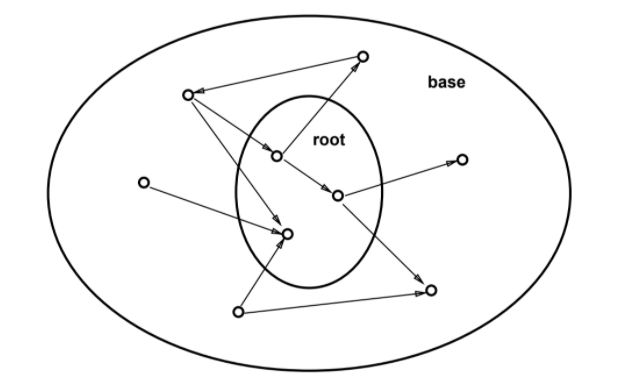
\includegraphics[width=0.7\textwidth]{root.png}  
\caption{Proširivanje root set-a u base set}
\end{figure}


\newpage
\section{Implementacija HITS algoritma}
Iterativno računamo autoritet-vrijednosti i hub-vrijednosti.
Sa $x^{(k)}$ i $y^{(k)}$ označimo vrijednost vektora $x$ odnosno $y$ u $k$-toj iteraciji. Iz jednadžbi (\ref{eq:2}) slijedi
\begin{equation}\label{eq:3}
cx^{(k+1)} = L^{T}Lx^{(k)}\hspace{1cm} cy^{(k+1)} = LL^{T}y^{(k)}˘
\end{equation}
uz početni uvjet
$x^{(0)} = y^{(0)} = (1, 1, \dots, 1)$, gdje je $c$ konstanta takva da vrijedi $||x||_{2} =1$ i $||y||_{2} =1$. Matricu $L^{T}L$ nazivamo matrica autoriteta, a matricu $LL^{T}$ nazivamo matrica hubova. Uočimo da su ove matrice simetrične.\\
Možemo zapisati algoritam:
\begin{enumerate}
\item Ulaz: Matrica linkova $L$
\item Inicijaliziramo $x^{(0)} = (1,1,\dots,1)$, $y^{(0)} = (1,1,\dots,1)$
\item Računaj $k$-tu iteraciju 
\begin{equation*}
x^{(k+1)} = L^{T}Lx^{(k)}\hspace{1cm} y^{(k+1)} = LL^{T}y^{(k)}˘
\end{equation*}
\item Normiraj dobivene vrijednosti
\begin{equation*}
x^{(k+1)} = \frac{x^{(k+1)}}{||x^{(k+1)}||_{2}}\hspace{1cm}y^{(k+1)} = \frac{y^{(k+1)}}{||y^{(k+1)}||_{2}}
\end{equation*}
\item Provjeri kriterij zaustavljanja
\begin{itemize}
\item Ako kriterij zaustavljanja nije zadovoljen, idi na 3, korak
\item Ako je kriterij zaustavljanja zadovoljen, završi
\end{itemize}
\item Izlaz: Vektori vrijednosti autoriteta, odnosno hubova, $x$ i $y$
\end{enumerate}
$i$-ta komponenta vektora $x$ predstavlja autoritet-vrijednost web stranice $p_{i}$, a $i$-ta komponenta vektora $y$ predstavlja hub-vrijednost web stranice $p_{i}$.

\newpage
\subsection{Implementacija HITS-a u Octaveu}
\begin{lstlisting}
function[] = hits(L, W,  n)
C = zeros(n,n);
R = zeros(n,n);
k = 0; 
eps = power (10, -5); 
xp = ones(n, 1); 
yp = ones(n, 1);
x = zeros(n,1);
y = zeros(n,1);
con = 1;
X = (L')*L; 
Y = L*(L');

while con
 x = X*(xp);
 x/=norm(x);
 y = Y*(yp);
  y/=norm(y);
   if norm(x-xp) < eps && norm(y-yp) < eps
     con = 0;
   else
     xp=x;
     yp=y;
     ++k;
   endif
endwhile

[x_sort, ix] = sort(x, 'descend');
[y_sort, iy] = sort(y, 'descend');

disp("Prvih dvadeset autoriteta ");
for i = 1:20
  disp(W(ix(i)));
endfor
disp("Prvih dvadeset hubova ");
for i = 1:20 
  disp(W(iy(i)));
endfor
\end{lstlisting}

\subsection{Rezultati}
Prikazujemo rezultate naše implementacije HITS algoritma
\subsection{Upit $\sigma =$ "california"}
Algoritam je izveden na skupu web stranica koji je nastao postupkom opisanim u (\ref{sec:1}). Podaci su preuzeti sa \url{http://www.cs.cornell.edu/courses/cs685/2002fa/}.
\begin{table} [h!]
\begin{tabular}{c|c|l}
HITS&Indgr&URL\\
\hline
1 & 2 & http://www.ca.gov/ \\
2 & 6 & http://www.sen.ca.gov/ \\
3 & 8 & http://www.assembly.ca.gov/\\
4 & 3 & http://www.leginfo.ca.gov/calaw.html\\
5 & 1 & http://www.yahoo.com/\\
6 & 11 & http://www.house.gov/\\
7 & 12 & http://www.fedworld.gov/\\
8 & 26 & http://www.lao.ca.gov/\\
9 & 24 & http://whttp://www.dot.ca.gov/\\
10 & 42 & http://www.courtinfo.ca.gov/\\
11 & 9 & http://www.epa.gov/\\
12 & 19 & http://www.census.gov/\\
13 & 5 & http://www.berkeley.edu/\\
14 & 21 & http://www.lycos.com/\\
15 & 41 & http://www.ss.ca.gov/\\
16 & 27 & http://www.caltech.edu/\\
17 & 23 & http://goldmine.cde.ca.gov/\\
18 & 24 & http://www.excite.com/\\
19 & 56 & http://www.ftb.ca.gov/\\
20 & 62 & http://www.csun.edu/
\end{tabular}
\caption{Rangiranje autoriteta za upit "california"}
\end{table}

\begin{table} [h!]
\begin{tabular}{c|c|l} 
HITS&Outdgr&URL\\
\hline
1 & 1 & http://www.water.ca.gov/www.gov.sites.html \\
2 & 24 & http://www.llnl.gov/OCM/Go\textunderscore To.html\\
3 & 3 & http://www.ca.gov/s/search/servers.html\\
4 & 5 & http://california.findlaw.com/CA10\textunderscore california\textunderscore governemnt/index.html\\
5 & 28 & http://www.occn.org/links.htm\\
6 & 13 & http://www5.onramp.net/~smcgarry/argonaut/caform.htm\\
7 & 103 & http://www.cyberg8t.com/mlms/Program.html\\
8 & 14 & http://www.siscr.cz/db/abcd/fil151.html\\
9 & 41 & http://kerncounty.com/rma/links.htm\\
10 & 40 & http://www.autoaccident.com/calres.html\\
11 & 72 & http://www.mother.com/~minao/lunrpage/\\
12 & 116 & http://www.research.digital.com/SRC/virtual-tourist/final/CaliforniaGov-state.html\\
13 & 2 & http://www.igs.berkeley.edu:8880/library/cgpp.html\\
14 & 74 & http://www.ci.torrance.ca.us/city/dept/library/GOVERN.HTM\\
15 & 15 & http://www.ilrg.com/gov/ca.html\\
16 & 63 & http://www.nocall.org/calif.html\\
17 & 16 & http://www.pirg.org/calpirg/links.htm\\
18 & 97 & http://www.cccd.edu/dis/gov.html\\
19 & 238 & http://www.calbar.org/2lin/2gov.htm\\
20 & 12 & http://www.asiadragons.com/education/north\textunderscore america/united\textunderscore states/california/
\end{tabular}
\caption{Rangiranje hubova za upit "california"}
\end{table}
\newpage
\subsection{Stranice slične k $p$ ='www.epa.gov'}
Algoritam je izveden na skupu web stranica nastalim postupkom opisanim u (\ref{sec:2}). Podaci su preuzeti sa \url{http://www.cs.cornell.edu/courses/cs685/2002fa/}.
\newpage
\begin{table} [h!]
\begin{tabular}{c|c|l}
HITS&Indgr&URL\\
\hline
1 & 2 &  http://www.epa.gov/\\
2 & 3 & http://www.yahoo.com/\\
3 & 4 & http://www.noaa.gov/\\
4 & 169 & http://www.usitc.gov/\\
5 & 83 & http://www.nrc.gov/\\
6 & 72 & http://www.nps.gov/\\
7 & 133 & http://www.fema.gov/\\
8 & 21 & http://lcweb.loc.gov/homepage/lchp.html\\
9 & 134 & http://www.iadb.org/\\
10 & 5 & http://www.mckinley.com/\\
11 & 13 & http://www.lycos.com/\\
12 & 222 & http://www.exim.gov/\\
13 & 223 & http://www.nara.gov/\\
14 & 2 & http://www.epa.gov\\
15 & 325 & http://www.clark.net/pub/peace/PeaceCorps.html\\
16 & 255 & http://www.un.org/\\
17 & 224 & http://govinfo.kerr.orst.edu/\\
18 & 182 & http://www.irs.ustreas.gov/\\
19 & 283 & http://www.ustr.gov/\\
20 & 9 & http://www.doc.gov/
\end{tabular}
\caption{Rangiranje autoriteta za stranicu "www.epa.gov"}
\end{table}
\newpage

\begin{table} [h!]
\begin{tabular}{c|c|l}
HITS&Outdgr&URL\\
\hline
1 & 1 & http://cyberspud.com/gov.html\\
2 & 21 & http://www.law.vill.edu/Fed-Agency/fedwebloc.html\\
3 & 22 & http://www.law.vill.edu/Fed-agency/fedwebloc.html\\
4 & 12 & http://tor-pw1.netcom.ca/~dhera/usagov.html\\
5 & 28 & http://www.kcc.state.ks.us/energy/links.htm\\
6 & 3 & http://www.phoenix.net/~blp/misc.html\\
7 & 41 & http://www.deq.state.la.us/other\textunderscore st.htm\\
8 & 11 & http://sio.ucsd.edu/sp\textunderscore progs/cetc/whc/c\textunderscore monitoring/inven.html\\
9 & 10 & http://kierkegaard.ifas.ufl.edu/\\
10 & 9 & http://apu.edu/~rconover/bookmark.html\\
11 & 52 & http://neon.mems.cmu.edu/MSE/other.html\\
12 & 44 & http://www.trans-action.com/websites.htm\\
13 & 48 & http://www.state.nc.us/EHNR/ee/links/eebkmks.htm\\
14 & 7 & http://www-sgc.colorado.edu/resources/dans\textunderscore resources.html\\
15 & 14 & http://www.imt.net/~dcouncil/envgov.html\\
16 & 2 & http://www.ridgeco.com/kzenv.html\\
17 & 34 & http://www.media-wave.com/Bookmarks/Env.html\\
18 & 80 & http://www.nes-inc.com/links.htm\\
19 & 57 & http://www.holonet.net/strategies/EarthRise/INTERNET-RESOURCES2\\
20 & 79 & http://www.ecotradenet.com/book1.htm
\end{tabular}
\caption{Rangiranje hubova za web stranicu "www.epa.gov"}
\end{table}


\newpage
\section{Sličnost s bibliometrijskom analizom}
Bibliometrija se bavi kvantitavnim proučavanjem pisanih dokumenata i pojava kao što su produktivnost autora, citiranje, disperzija članaka, učestalost riječi. \\
Ko-citacija dokumenata $a$ i $b$ je mjera sličnosti koja se definira kao frekvencija citiranja ta dva dokumenta, tj. broj dokumenata koji citiraju dokumente $a$ i $b$. Što je veći broj dokumenata koji citiraju $a$ i $b$, njihova je ko-citacija veća pa je veća vjerojatnost da su $a$ i $b$ semantički slični.\\
Slično, ko-referenca dokumenata $a$ i $b$ je mjera sličnosti koje se definira kao broj dokumenata na koje $a$ i $b$ imaju referencu. Ako $a$ i $b$ imaju veću ko-referencu, veća je vjerojatnost da $a$ i $b$ obrađuju sličnu temu.\\
Na sličan način možemo definirati mjere sličnosti između autoriteta, odnosno hubova.
\subsection{Autoriteti i ko-citacije}
Ako na web stranice $p_i$ i $p_j$ pokazuje veći broj stranica, vjerojatnije je da su one na neki način slične.
Za web stranice $p_i$ i $p_j$ definiramo ko-citacije kao broj web stranica koje pokazuju na $p_i$i $p_j$. Matrično se ovo može zapisati kao
\begin{equation}
C_{ij} = \sum_{k} L_{ki}L_{kj} = \sum_{k}(L^{T})_{ik}L_{kj} = (L^{T}L)_{ij}
\end{equation}
uz $C_{ii} = 0$. Također vrijedi simetrija, tj. $C_{ij} = C_{ji}$.\\
Označimo sa $d_{i}$ stupanj ulaznosti stranice $p_{i}$. $d_{i}$ možemo računati kao
\begin{equation}
d_{i} = \sum_{k}L_{ki} = \sum_{k}L_{ki}L_{ki} = (L^{T}L)_{ii}
\end{equation}
jer je $L_{ki} = L_{ki}^2$ jer je $L_{ki} =1$ ili  $L_{ki} = 0$.\\
Definiramo matricu stupnjeva ulaznosti $D$:
\begin{equation}
D = diag(d_{i},d_{2}, \dots , d_{n})
\end{equation}
Tada matrica autoriteta ima sljedeću strukturu:
\begin{equation}
L^{T}L = D + C
\end{equation}
odnosno, matrica autoriteta je zbroj matrice ko-citacija i matrice stupnjeva ulaznosti.
\subsection{Hubovi i ko-reference}
Za web stranice $p_i$ i $p_j$ definiramo ko-reference kao broj web stranica na koje pokazuju $p_i$i $p_j$. Matrično se ovo može zapisati kao
\begin{equation}
R_{ij} = \sum_{k} L_{ik}L_{jk} = \sum_{k}L_{ik}(L^{T})_{kj} = (LL^{T})_{ij}
\end{equation}
uz $R_{ii} = 0$. Također vrijedi simetrija, tj. $R_{ij} = R_{ji}$.\\
Označimo sa $o_{i}$ stupanj izlaznosti stranice $p_{i}$. $o_{i}$ možemo računati kao
\begin{equation}
o_{i} = \sum_{k}L_{ik} = \sum_{k}L_{ik}L_{ik} = (LL^{T})_{ii}
\end{equation}
jer je $L_{ik} = L_{ik}^2$ jer je $L_{ik} =1$ ili  $L_{ik} = 0$.\\
Definiramo matricu stupnjeva izlaznosti $O$:
\begin{equation}
O = diag(o_{i},o_{2}, \dots , o_{n})
\end{equation}
Tada matrica autoriteta ima sljedeću strukturu:
\begin{equation}
LL^{T} = O + R
\end{equation}
odnosno, matrica hubova je zbroj matrice ko-referenca i matrica stupnjeva izlaznosti.

Također, imamo nejednakost:
\begin{equation}
    max \{0, o_{i} + o_{k} - n\} \leq R_{ik} \leq min\{o_{i}, o_{k}\}
\end{equation}

Direktna posljedica ove tvrdnje je $R_{ik} = 0$ ako $o_{i} = 0$ ili $o_{k} = 0$. Dakle, ako web stranica $p_{i}$ stupanj izlaznosti 0, tada je i-ti red $LL^{T}$ jednak 0. Iz jednadžbe (\ref{eq:3}), slijedi da hub score mora biti 0.

\newpage
\section{Konvergencija algoritma}
Primijetimo da je $L^{T}L = (LL^{T})^{T}$. Stoga, matrice $L^{T}L$ i $LL^{T}$ imaju iste svojstvene vrijednosti. Kako su to realne i simetrične matrice, njihove svojstvene vrijednosti su također realne.\\
Neka su $\lambda_{1}$, $\lambda_{2}$, $\dots$, $\lambda_{n}$ svojstvene vrijednosti ovih matrica poredane padajuće po apsolutnoj vrijednosti, tj. vrijedi $|\lambda_{1}|\geq |\lambda_{2}|\geq \dots \geq |\lambda_{n}|$. Pretpostavimo da vrijedi $|\lambda_{1}| > |\lambda_{2}|$
Svojstvenu vrijednost $\lambda_{1}$ nazivamo dominantna svojstvena vrijednost.

\begin{theorem}
Nizovi $x^{(1)}, x^{(2)}, x^{(3)}\dots$ i $y^{(1)}, y^{(2)}, y^{(3)}\dots$ konvergiraju limesima $x^{*}$ i $y^{*}$.
\end{theorem}
\begin{proof}
Neka je $G = (V, E)$, gdje je $V = \{k_1 \ldots k_{n}$ i neka je A adjunktna matrica grafa G. Element na mjestu $(i,j)$ jednak je 1 ako je $(p_{i}, p_{j})$ brid grafa $G$, a 0 inače. Lako se provjeri da operacije $I$ i $O$ mogu biti napisane kao $x \leftarrow A^{T}y$ i $y \leftarrow Ax$, redom. Tada je $x_{k}$ jedinični vektor u smjeru $(A^{T}A)^{k-1}A^{T}z$, a $y_{k}$ jedinični vektor u smjeru $(AA^{T})^{k}z$.

Linearna algebra nam kaže da ako je $M$ simetrična $nxn$ matrica i vektor $v$ nije ortogonalan svojstvenom vektoru $\omega_{1}(M)$ tada jedinični vektor u smjeru $M{k}v$ konvergira prema $\omega_{1}(M)$ kako se k povećava. Također, M ima samo nenegativne ulaze, pa glavni svojstveni vektor od $M$ ima samo nenegativne vrijednosti.

Posljedično, z nije ortogonalan $\omega_{1}(AA^{T})$ pa tada niz $\{y_{k}\}$ konvergira prema $y^{*}$.
Na sličan način se pokaže da ako je $\lambda_{1} \neq 0$, tada $A^{T}z$ nije ortogonalan na $\omega_{1}(AA^{T})$. Iz toga slijedi da niz $\{x_{k}\}$ konvergira prema $x^{*}$.
\end{proof}

Dokaz ovog teorem daje sljedeći rezultat.
\begin{theorem}
$x^{*}$ je dominantni svojstveni vektor matrice $L^{T}L$, a $y^{*}$ je dominantni svojstveni vektor matrice $LL^{T}$.
\end{theorem}

\newpage
\section{Vjerojatnosna analiza}
Analizirali smo strukturu autoriteta i hubova. Rezultati jednadžbe LALA pokazuju zanimljivu vezu između ko-citacija i stupnja ulaznosti: općenito, čvorovi s velikim izlaznim stupnjem će imati velike ko-citacije s ostalim čvorovima samo zato jer imaju više ulaznih linkova/bridova. Slično, veliku ko-referencu povezujemo s velikim izlaznim brojem linkova.

Ovakva intuicija se može precizirati ako pretpostavimo da (web) graf ima nasumično raspoređen graf fiksnog stupnja te koristeći vjerojatnosnu analizu na očekivanim vrijednostima ko-citacije i ko-reference. 
Općenito govoreći, web graf je nasumičan graf - milijuni pojedinaca i organizacija kreiraju web stranice za različite svrhe. Predlaže se da je web bolje opisan nasumičnim grafom fiksnog supnja, unutar kojeg su čvorovi stupnjeva $\{d_{1} \ldots d_{n}\}$ prvo dani, a bridovi su nasumično raspoređeni između čvorova koji podliježu ograničenjima stupnjeva čvorova.
Stoga imamo sljedeću tvrdnju:
\begin{prop}
Prosječna vrijednost ko-citacija dana je formulom
\begin{equation} \label{eq:4}
\langle C_{ik}\rangle = \frac{d_{i}d_{k}}{n-1}
\end{equation}
\end{prop}
\begin{proof}
Pretpostavimo da je $d_{i} \geq d_{k}$. Tada iz jednadžbe (\ref{eq:3}) vidimo da ima barem $d_{k}$  elemenata različitih od 0, što je INNER PRODUCT i-tog retka i k-tog stupca matrice L.Promotrimo slučaj kada je q-ti red u k-tom stupcu jednak 1. Vjerojatnost da je vrijednost u i-tom stupcu jednaka 1 jest:
\begin{equation*}
    P(L_{qi} = 1) = \frac{C_{n-2}^{d_{i}-1}}{C_{n-1}^{d_{i}}} = \frac{d_{i}}{n-1}
\end{equation*}
Ovdje je $C_{n-1}^{d_{i}}$ ukupan broj svih mogućih rasporeda $d_{i}$ jedinica u i-tom stupcu, a $C_{n-2}^{d_{i}-1}$ je ukupan broj svih mogućih rasporeda ako je jedinica u retku q.
Dakle,
\begin{equation*}
    \langle C_{ik}\rangle = \sum_{q} \langle L_{qi}, L_{qk} \rangle= \sum_{q}^{d_{k}} \langle L_{q} \rangle = d_{k} * P(L_{qi} = 1)
\end{equation*}
odakle slijedi (\ref{eq:4})
\end{proof}

Iz ove analize, vidimo da će vrh $i$ s velikim izlaznim stupnjem $d_{i}$ imati veliku ko-citaciju s drugim vrhovima, a ako to usporedimo s vrhom $j$ koji ima manji izlazni stupanj $d_{j}$ tj. ako je $d_{i} > d_{j}$, tada je:
\begin{equation*}
    \langle C_{ik} \rangle > \langle C_{jk} \rangle  \hspace{1cm} \forall k, k \neq i, k \neq j
\end{equation*}

Iz ove probabilističke jednadžbe, zaključujemo da je $C_{ik}$ veći od $C_{jk}$ većinu vremena, što nije nužno istina u svakom slučaju.  
Praktičnosti radi, kažemo da \emph{u prosjeku} vrijedi $C_{ik} \gtrsim C_{jk}$.

Na sličan se način ova analiza može primijeniti za izlazni stupanj i ko-referencu hubova matrice $LL^{T}$.
Imamo:
\begin{equation*}
    \langle R_{ik} \rangle = \frac{o_{i} o_{k}}{n-1}
\end{equation*}
Ako je $o_{i} > o_{j}$, tada $\langle R_{ik} \rangle > \langle R_{jk} \rangle$, odnosno kažemo da  $R_{ik} \gtrsim R_{jk}$. vrijedi \emph{u prosjeku}.





\section{Average case analiza}
Zbog dosadašnjih analiza, sada možemo zamijeniti matricu autoriteta njihovim prosječnim vrijednostima. 
\begin{theorem}
Matrica autoriteta $L^{T}L$ u prosječnom slučaju, uz uvjet 
\begin{equation}
    d_[i]+d_{j}<n+1
\end{equation} za svaki $i,j$ ima sljedeće svojstvene vrijednosti i svojstvene vektore:
\begin{enumerate}
\item Za svojstvene vrijednosti vrijedi
\begin{equation}
\lambda_{1} > \hat{d_{1}}>\lambda_{2}>\hat{d_{2}}>\dots >\lambda_{n}>\hat{d_{n}}
\end{equation}
\item k-ti svojsteni vektor je
\begin{equation} \label{eq:15}
\textbf{u}_{k}= \left(\frac{d_{1}}{\lambda_{k}-\hat{d_{1}}},\frac{d_{2}}{\lambda_{k}-\hat{d_{2}}},\dots, \frac{d_{n}}{\lambda_{k}-\hat{d_{n}}} \right)^{T}
\end{equation}
\end{enumerate}
Web stranice indeksiramo tako da je $d_{1}>d_{2}>\dots>d_{n}$ i vrijedi $\hat{d_{i}} = d_{i} - \frac{d_{i}^{2}}{n-1}$.
\end{theorem}

\begin{figure}[ht!]
\centering
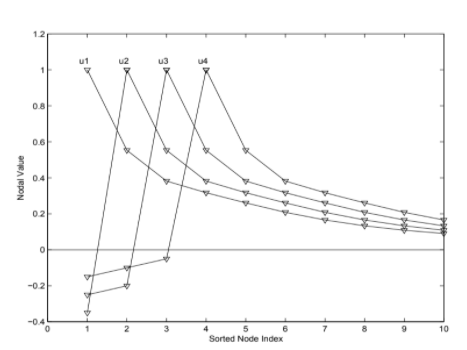
\includegraphics[width=0.7\textwidth]{svvektori.png}  
\caption{Svojstveni vektori jednadžbe \label{eq:15}}
\end{figure}

\begin{proof}
Koristeći izraz (\ref{eq:4}), prosječna matrica autoriteta je
\begin{equation}
\langle L^{T}L\rangle = \langle D \rangle + \langle C \rangle = diag(\hat{d_{1}}, \dots , \hat{d_{n}}) + \frac{1}{n-1} dd^{T}
\end{equation}
\end{proof}
Analogan rezultat vrijedi za matricu hubova $LL^{T}$.
\begin{corollary}
Elementi dominantnog vektora $\textbf{u}_1$ su padajući, tj. za $i<j$ vrijedi 
\begin{equation}
u_{1}(i)-u_{1}(j)>0
\end{equation}
\end{corollary}
\begin{proof}
\begin{equation}
u_{1}(i)-u_{1}(j) = \frac{d_{i}}{\lambda_{1} - \hat{d_{i}}} - \frac{d_{j}}{\lambda_{1} - \hat{d_{j}}} = \frac{(d_{i}-d_{j})[\lambda_{1}-d_{i}d_{j}(n-1)]}{(\lambda_{1}-\hat{d_{i}})(\lambda_{1}-\hat{d_{j}})} >0
\end{equation}
jer je
\begin{equation}
\lambda_{1} - d_{i}d_{j}(n-1) \overset{\mathrm{(\ref{eq:6})}}{>}\hat{d_{i}} - d_{i}d_{j}(n-1) = d_{i}(1-(d_{i}+d_{j})/(n-1))\overset{\mathrm{(\ref{eq:5})}} {>}0
\end{equation}
\end{proof}
Iz ovo korolara, možemo zaključiti da je, u prosječnom slučaju, poredak web stranica po autoritet-vrijednostima jednak poretku po stupnju ulaznosti.\\
Analogan rezultat vrijedi za matricu hubova $LL^{T}$, tj. u prosječnom slučaju, poredak web stranica po hub-vrijednosti jednak je poretku po stupnju izlaznosti.

\newpage

\section{Svojstva HITS algoritma}

Nekoliko zanimljivih rezultata slijedi direktno iz prethodnog teorema:
\begin{enumerate}
    \item \textbf{Organiziranje web stranica.} Rangiranje autoriteta, je u prosjeku, identično kao rangiranje stranica pomoću ulaznih stupnjeva. Kako bi nam bilo to jasnije, imamo sljedeću tvrdnju:
    \begin{corollary}
    Elementi glavnog svojstvenog vektora $u_{1}$ monotono padaju.
    \end{corollary}
    \begin{proof}
    Za svaki $i < j$:
    \begin{equation*}
        u_{1} (i) - u_{1}(j) = \frac{d_{i}}{\lambda_{1} - \hat{d_{i}}} - \frac{d_{j}}{\lambda_{1} - \hat{d_{j}}} = \frac{(d_{i} - d_{j})[\lambda_{1} - \frac{d_{i}d_{j}}{n-1}]}{(\lambda_{1} - \hat{d_{i}})(\lambda_{1} - \hat{d_{j}})} > 0
    \end{equation*}
    \end{proof}
     Iz ovoga zaključujemo da je rangiranje web stranica pomoću njihovih autority scorova isto kao i rangiranje prema ulaznim stupnjevima. Praktična primjena ovih rezultata jest da je jednostavno brojanje ulaznih bridova kao algoritam rangiranja učinkovito i efikasno.
     
     \item \textbf{Jedinstvenost.} Ako je $d_{1} > d_{2}$, tada je glavni svojstveni vektor $L^{T}L$ jedinstven i različit od drugog glavnog svojstvenog vektora.
     
     \item \textbf{Konvergencija}. Konvergencija HITS algoritma može biti dosta brza. Početni vektor $x^{(0)} = (1 \ldots 1) $ ima vrlo malo preklapanja s ostalim svojstvenim vektorima $(x^{(0)} * u_{k}, k > 1)$ jer svi oni sadrže negativne vrijednosti čvora.
     Koristeći $L^{T}L = \lambda_{1}u_{1}u_{1}^{T} + \lambda_{2}u_{2}u_{2}^{T} + \ldots $ nakon k iteracija, imamo:
     \begin{equation*}
         x^{(k)} = c_{1}\lambda_{1}^{k}u_{1} +  c_{2}\lambda_{2}^{k}u_{2} + \ldots 
     \end{equation*}
     gdje je $c_{2} \ll c_{1}$ zbog malih preklapanja između $x^{(0)}$ i $u_{2}$
     
     \item \textbf{Web zajednice.} HITS algoritam se uvijek koristio za identificiranje mnogih web zajednica koristeći različite svojstvene vrijednosti. Glavni svojstveni vektor definira dominantnu web zajednicu. Svaki sporedni svojstveni vektor definira dvije zajednice, jednu s nenegativnim $\{i | u_{k}(i) \geq 0\}$ i drugu s negativnim vrijednostima $\{i | u_{k}(i) < 0\}$
\end{enumerate}

\newpage
\begin{thebibliography}{9}
\bibitem{prvi} 
Chris Ding, Honqyuan Zha, Xiaofeng He, Parry Husbands, Horst Simon
\textit{Link Analysis: Hubs and Authorities on the World Wide Web}. 
\\\texttt{http://ranger.uta.edu/~chqding/papers/hits5.pdf}
2001.

\bibitem{drugi} 
Soumen Chakrabarti, Byron E.Dom, David Gibson, Jon Kleinberg, Ravi Kumar, Prabhakar Raghaan, Sridhar Rajagopalan, Andrew Tomkins
\textit{Mining the Link Structure of the World Wide Web}. 
\\\texttt{https://www.cs.cornell.edu/home/kleinber/ieee99-web.pdf}
1999.

\bibitem{treci} 
Jon M. Kleinberg
\textit{Authoritative Sources in a Hyperlinked Environment}. 
\\\texttt{https://www.cs.cornell.edu/home/kleinber/auth.pdf}

\end{thebibliography}


\end{document}